% !TeX spellcheck = en_US

\documentclass{../UTNetLab}

\title{UDP and Its Applications}
\labnumber{5}
\newcommand\reference{
   S. Panwar, S. Mao, J.-dong Ryoo, and Y. Li, “UDP and its applications,” in TCP/IP Essentials: A Lab-Based Approach, Cambridge: Cambridge University Press, 2004, pp. 100–110.
}

\begin{document}
\section*{Objectives}
\begin{itemize}
    \item Study \textbf{socket} as a traffic generator, in terms of its features and command line options.
    \item Study the User Datagram Protocol.
    \item IP fragmentation.
    \item MTU and path MTU discovery.
    \item UDP applications, using the Trivial File Transfer Protocol as an example.
    \item Compare UDP with TCP, using TFTP and the File Transfer Protocol (FTP).
\end{itemize}

\part{Using the \texttt{socket} Program}
\label{sec:schema}
In this lab, you will not need to a router, only two hosts and one hub to connect two host together as show in \hyperref[fig:5.0]{Figure~5.0} and \hyperref[tab:5.0]{Table~5.0}.
Also you can use Figure~1.3.
\begin{table}[H]
    \caption{Host IP addresses for \hyperref[fig:5.0]{Figure~5.0}}
    \label{tab:5.0}
    \centering
    \begin{tabular}{ *2c|*2c }
        \hline \hline
        \multicolumn{2}{c|}{Host\textsubscript{A} (h0)} & \multicolumn{2}{c}{Host\textsubscript{B} (h1)}                            \\
        Name                                            & IP Address                                     & Name & IP Address        \\
        \hline
        h0                                              & 128.238.61.100/24                              & h1   & 128.238.61.101/24 \\
        \hline \hline
    \end{tabular}
\end{table}

\begin{figure}[H]
    \centering
    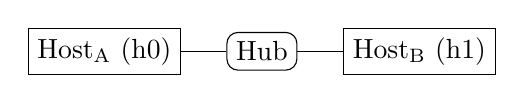
\begin{tikzpicture}
        \node[draw] (h1) at (-2,0){Host\textsubscript{A} (h0)};
        \node[draw,rounded corners] (hub) at (0,0){Hub};
        % \node[draw,rounded corners] (router) at (0,0){Router};
        % \node[draw,rounded corners] (hub1) at (2,0){Switch 1};
        \node[draw] (h0) at (2,0){Host\textsubscript{B} (h1)};

        \draw (h0) -- (hub) -- (h1);
    \end{tikzpicture}
    \caption{Simple router experiment (Figure~5.0)}
    \label{fig:5.0}
\end{figure}

\section{Socket Operation}
Use the following commands in the \textit{h0} and the \textit{h1} as client and server host to observe the basic operation of \lstbash{socket}\footnote{Basic command is \lstbash{sock} use alternative \lstbash{socket} (rename of \lstbash{sock})} and \lstbash{echo} service.
\begin{lstlisting}[emph={host, h1,netlab},morekeywords={[3]echo}]
socket [-u] host echo@\footnote{Type any text in socket and press enter.}@
socket -s 5555 #on h1
socket -i -n3 -w2048 128.238.61.101 5555 # on h0
    \end{lstlisting}

\begin{report}
    \item Explain the operation of each command.
\end{report}

\section{\texttt{socket -h}}
Study various options associated with the \lstbash{socket} program.
A brief list of options can be displayed by typing \lstbash{socket}.
More detailed discussion on socket can be found in Appendix~C of [5] in the reference book.

\section{Segment Size}
While running \lstbash{tcpdump -nv &} or \lstbash{wireshark} on the \textit{h0} or the \textit{h1} machine, execute the following command with different values of size (i.e.\  the size of the datagram) on the \textit{h0}.

\begin{lstlisting}[emph={size, h1,netlab},morekeywords={[3]echo}]
socket -u -i -n1 -w size 128.238.61.101 echo
    \end{lstlisting}

The \lstbash{-u} option is used to send UDP datagrams rather than TCP segments.

Increase \textit{size} (i.e.\  the size of the datagram) until fragmentation occurs.

Use \lstbash{netstat -in} to find out the MTU of the Ethernet interface.

\begin{report}
    \item What is the maximum value of \textit{size} for which the UDP datagram can be sent without IP fragmentation?
    Justify your answer with the \lstbash{netstat} output.
\end{report}

\section{Datagram Fragmentation}
Capture the data packets generated by \lstbash[emph={h1.netlab},morekeywords={[3]src,host}]{tcpdump src host h1.netlab} command on the \textit{h1}.

\begin{lstlisting}[emph={h1,netlab},morekeywords={[3]echo}]
socket -u -i -n1 -w10000 128.238.61.101 echo # on h0
    \end{lstlisting}
Save the \lstbash{tcpdump} output for the lab report.

\begin{report}
    \item Explain the \lstbash{tcpdump} output in terms of the IP header fields that are used in fragmentation.

    \item When IP fragmentation occurs, only the first fragment has the UDP header.
    How do you verify this fact from the \lstbash{tcpdump} output?
\end{report}


\section{Maximum Datagram Size}
\label{sec:MaxDatagramSize}
While running \lstbash{tcpdump}, execute the following command on the \textit{h0} host with different values of size (for example 10000),
\begin{lstlisting}[emph={size, h1,netlab},morekeywords={[3]echo}]
socket -u -i -n1 -w size 128.238.61.101 echo # on h0
\end{lstlisting}
% socket -u -i -n1 -w65507 h1.netlab echo
in order to find out the maximum size of a UDP datagram that the system can send or receive, even when fragmentation is allowed.

\begin{report}
    \item What is the maximum size of user data in a UDP datagram that the system can send or receive, even when fragmentation is allowed?
\end{report}


\part{Path MTU Discovery Exercise}\label{sec:PMTUD}

\section{Discover path MTU}
Connect the routers and the hosts as shown in \hyperref[fig:5.5]{Figure~5.5} Change the IP addresses of all hosts accordingly.
Note that the router IP addresses are the same as their default.
Also you need to add route for all hosts to other subnets.

% Open console of  each router, enable {RIP} routing (See Section~4.6 of reference book).
% ifconfig interface_name mtu new_MTU_value.

Change the \texttt{MTU} of the \textit{ethernet1} interfaces of \textit{Router4} to 500 bytes.
\begin{lstlisting}[language={cisco}]
R1(config-if)# ip unreachables ! enables the router to send ICMP unreachable errors
R1(config-if)# ip mtu 500
! this command set ip layer mtu size
! the real packet has 20 byte ip header (or more depend on options value)
R1(config-if)# mtu 500 ! may be not supported (can see: mtu ?)
! this command set ethernet layer mtu size
    \end{lstlisting}

Test connectivity by \lstbash{ping}ing hosts in the other subnets.
After you can reach the
hosts in the other subnets, run \lstbash{tcpdump -nx} on your host.

Start a UDP socket server on the \textit{h1} host, using \lstbash{socket -u -s 5555}.
Then run the socket client from the \textit{h0}:
\begin{lstlisting}[emph={h1,netlab}]
socket -i -u -n10 -w400 -p5 128.238.62.101 5555
    \end{lstlisting}

\begin{table}[H]
    \caption{Router and Host IP addresses for \hyperref[fig:5.5]{Figure~5.5} (Table~5.5)}
    \centering
    \begin{tabular}{ *2c|*2c|*2c }
        \hline \hline
        \multicolumn{2}{c|}{Router} & \multicolumn{2}{c|}{Host\textsubscript{A} (h0)} & \multicolumn{2}{c}{Host\textsubscript{B} (h1)}                                                \\
        eth0                        & eth1                                            & Name                                           & IP Address        & Name & IP Address        \\
        \hline
        128.238.61.1/24             & 128.238.62.1/24                                 & h0                                             & 128.238.61.101/24 & h1   & 128.238.62.101/24 \\
        \hline \hline
    \end{tabular}
\end{table}

\begin{figure}[H]
    \centering
    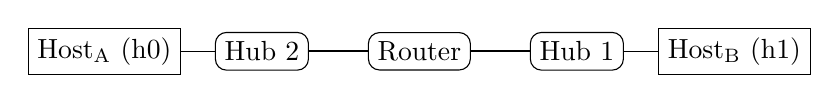
\begin{tikzpicture}
        \node[draw] (h1) at (-4,0){Host\textsubscript{A} (h0)};
        \node[draw,rounded corners] (hub2) at (-2,0){Hub 2};
        \node[draw,rounded corners] (router) at (0,0){Router};
        \node[draw,rounded corners] (hub1) at (2,0){Hub 1};
        \node[draw] (h0) at (4,0){Host\textsubscript{B} (h1)};

        \draw (h0) -- (hub1);
        \draw (h1) -- (hub2);
        \draw[thick] (hub1) -- (router);
        \draw[thick] (hub2) -- (router);
    \end{tikzpicture}
    \caption{The network setup for \nameref{sec:PMTUD} (Figure~5.5/Figure~4.10)}
    \label{fig:5.5}
\end{figure}

Observe the DF bit of the first datagram and that of the following datagrams.
Save the \lstbash{tcpdump} output for your lab report.

\begin{report}
    \item Explain the operation of path MTU discovery based on the \lstbash{tcpdump} outputs saved.

    \item Which ICMP message is used in path MTU discovery? Give the decimal value of each field of the captured ICMP message.

    \item What is the MTU of the destination network of the UDP datagram? Verify your answer using both the ICMP message and the IP fragmentation trace saved.
\end{report}

\part{Exercises with FTP and TFTP}
Use first network (section \nameref{sec:schema}) topology (\hyperref[fig:5.0]{Figure~5.0} or Figure~1.3) for this exercise.

We will study the performance of FTP and TFTP for file transfer between two machines.
By transferring the same file using these two protocols, we can compare the operations and performances of UDP and TCP.

Four files (\path{large.dum}, \path{med.dum}, \path{small.dum} and \path{thin.dum}) with random contents are stored in the \path{/home/netlab} directory and in the \path{/home/netlab}\footnote{We change original path (\path{/tftpboot}) to \path{/home/netlab} to be same as ftp user path.} directory of each host in the lab.
We will use the \lstbash{get} command to retrieve files from the \textit{h1} host.
When FTP is used, you need to change directory to \path{/home/netlab/} by \lstbash{cd /home/netlab} before retrieving the file.
If you don’t know how to use \lstbash{tftp}, refer to its manual page.


\section{TFTP and FTP}
In order to compare the transfer rates of FTP and TFTP, we will retrieve all large, med, small and thin files from the \textit{h1} server using FTP and TFTP, respectively.

First run First run the following \lstbash{tcpdump} command:
\begin{lstlisting}[emph={h0,h1,netlab},morekeywords={[3]host,and}]
tcpdump host 128.238.61.100 and 128.238.61.101
    \end{lstlisting}

You can use the redirect operator, \lstbash{>}, to save the \lstbash{tcpdump} output into a text file for large \lstbash{tcpdump} outputs and read it with \lstbash{less, grep, nano} or \lstbash{vim}.
For example you can change previous command into:
\begin{lstlisting}[emph={h0,h1,netlab,output,dump},morekeywords={[3]host,and}]
tcpdump host 128.238.61.100 and 128.238.61.101 > output.dump
    \end{lstlisting}

Now you should repeat this scenario for all files (\path{large.dum}, \path{med.dum}, \path{small.dum} and \path{thin.dum}) on the \textit{h0} machine.
\begin{lstlisting}[emph={h1,netlab},morekeywords={[2]get,quit}]
$ ls /etc/xinetd.d/ # see services in xinetd
$ tftp 128.238.61.101
tftp> get $filename # thin.dum, small.dum, med.dum, large.dum
tftp> quit
$ ftp 128.238.61.101 # Enter user and password -> netlab and netlab
ftp> ls
ftp> get $filename # thin.dum, small.dum, med.dum, large.dum
ftp> quit
    \end{lstlisting}
% Create \path{small.dum} with 10kB, \path{med.dum} with 1MB and \path{larg.dum} with 50MB.

Also, from the \lstbash{ftp} window, record the transfer rate (time) displayed.

Restart the above \lstbash{tcpdump} session.

\begin{report}
    \item Examining the saved \lstbash{tcpdump} output.
    Identify the starting and ending time of actual data transfer.
    Don’t include the time spent establishing the TCP connection.
    Calculate the time spent for data transfer.

    \item Compare the time with the value displayed in \lstbash{ftp} window.
    Are they consistent?
    If there exists any significant difference, what might be the reason?

    \item Now, from the second session, carefully determine the starting and ending time of data transfer for the \lstbash{tftp} program.

    \item Compare the time with the value displayed in \lstbash{tftp} window.
    Are they consistent?
    If there exists any significant difference, what might be the reason?

    \item By comparing the actual data transfer times of \lstbash{ftp} and \lstbash{tftp}, which of these two is faster, and why?
\end{report}

\section{TFTP Analysis}
Capture the packets that are exchanged during a \lstbash{tftp} session for the \path{/home/netlab/small.dum} file between \textit{h0} and the \textit{h1}, using:
\begin{lstlisting}[emph={h0,h1,netlab},morekeywords={[3]host,and}]
tcpdump -x host 128.238.61.100 and 128.238.61.101
    \end{lstlisting}
Observe the protocol in action.
Analyze various types of TFTP messages.
Save \lstbash{tcpdump} output for the lab report.

\begin{report}
    \item List all the different types of packets exchanged during the \lstbash{tftp} session.
    Compare them with the TFTP message format in \hyperref[fig:5.3]{Figure~5.3} of reference book.

    Why does the server’s port number change?

    \item In most cases, \lstbash{tftp} service is restricted.\footnote{This is not the case in our lab, where we deliberately enabled the \lstbash{tftp} service and use it as a tool to study the UDP protocol.}
    Why is \lstbash{tftp} service not generally available to users? At least write two problem of \lstbash{tftp} protocol.

    \item In \autoref{sec:MaxDatagramSize}, we found the maximum size of a UDP datagram in your machine.
    With \lstbash{tftp}, which uses UDP, we transferred a file larger than the maximum UDP datagram size.
    How do you explain this?
\end{report}

\section{FTP Small File}
Repeat the above experiment, but use \lstbash{ftp}.
Capture a trace of the packets exchanged when downloading the \path{/home/netlab/small.dum} file using \lstbash{ftp}.

Examine the port numbers used.

\begin{report}
    \item How many well-known port numbers were used?
    Which machine used the well-known port numbers?
    What were the other machine’s port numbers?

    \item As can be seen from the \lstbash{tcpdump} output, FTP involves two different connections, \texttt{ftp-control} and \texttt{ftp-data}.
    Why are two different connections used, instead of one connection?
\end{report}

\section{FTP Debug}
Run \lstbash{ftp} on the \textit{h0} using the debug mode: \lstbash[emph={h0,h1,netlab}]{ftp -d 128.238.61.101}.

After logging into the \textit{h1} host, type \lstbash{dir /home/netlab/small.dum} in the \lstbash{ftp} window.

Then type \lstbash{quit} to terminate the \lstbash{ftp} session, and save the \lstbash{ftp} window output.

\begin{report}
    \item Submit what you saved in this exercise, explaining each line of the output.
    Explain how the \lstbash{PORT} command works.
    Which connection, the control connection or the data connection, did the server send the response (the \lstbash{LIST} output) on?
\end{report}

\end{document}